\chapter{実験内容}
\section{モデルによる違い}
 本研究ではMagentaで用意されている2つの学習モデルを用いた。以下に示すモデルを用いて楽曲制作をそれぞれ行い,比較,検証する.\\

\subsection{MelodyRNN}
 MelodeRNNは楽曲のメロディを制作するモデルである.MelodyRNNである3つのモデルを以下に示す.\\
(1) basic\_rnn\\
 前の状態を保持し,これを記憶または忘却する.時系列を学習することにより,次の音の予測を可能にしている.Lookback\_rnnとAttention\_rnnはこれを基に機能を追加したものである.\\
\begin{figure}[!ht]
    \begin{screen}
    \begin{center}
        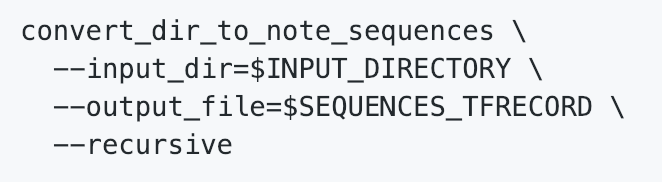
\includegraphics[scale=0.7, clip]{./img/Notesequence_make.png}
        \caption{NoteSequenceの作成}
        \label{fig:NoteSequenceの作成}
    \end{center}
    \end{screen}
\end{figure} \\
(2) lookback\_rnn\\
 Basic\_rnnを基に,1小節前と2小節前の音,拍数,前の小節の繰り返しかどうかの情報を与え,音楽の流れを掴もうとするもの.\\
(3) attention\_rnn\\
 basic\_rnnを基に,過去の情報を予測結果に加えてこれによる繰り返しを捉えるもの.\\

\subsection{PolyphonyRNN}
 複数の同時音のモデリングが可能になっており,複数音の響きを1つのかたまりとして捉えて学習しているモデルである.このモデルを使用することで,伴奏も含めた楽曲の生成が可能である。\\
\\
上記のモデルを用いて制作を行い,それぞれの違いと有用性について検証する.
\section{学習回数による違い}
 学習回数を変更して楽曲制作を行い,それぞれの違いと有用性について検証する.
\section{ノード数による違い}
 ノード数を変更して楽曲制作を行い,それぞれの違いと有用性について検証する.